\chapter{Concept and Design}
\label{cha:conceptanddesign}

This chapter focuses on the central concept for user segmentation in financial transaction networks. It is designed in the form of a data science pipeline, which consists of three primary stages of data processing. The purposes and contents of each stage will be covered below in detail. 

One of the main contributions of the current thesis is the first stage of the pipeline. It is represented by new modification of Node2vec framework for unsupervised network feature engineering taking into account dynamic nature of a network and remote structural homogeneity. The stage will be discussed and explained in this chapter with illustrations to allow a reader to fully comprehend the idea. The second stage of the data processing pipeline reduces dimensions of the data and serves as a preparation for the third final stage. The third stage is clustering in the low-dimentional feature space. Each stage was implemented as a set of relevant unsupervised or semi-supervised state-of-the-art machine learning techniques, which led to branch structure of the pipeline. The output is the set of clusters achieved the best magnitudes of the evaluation measures among different pipeline's branches.

The basic requirements for the user segmentation pipeline are listed below:
\begin{itemize}
  \item The pipeline should be able to read and process the network data from anonymized financial transaction data set with time and result into a set of clusters of similar users. 
  \item The pipeline should consider structures of the local neighbourhoods of the users, time of committed transactions and the global structural attribute of the underlying network.
  \item The pipeline should provide several techniques at each processing stage and output clusters evaluation values from every possible successive combination of techniques (branch).
\end{itemize}

\section{Concept}
\label{Concept}
~\autoref{fig:Fig28} depicts the main stages of the concept. The input data should be in the form of a structured set of transactions with the minimum required fields: sender, receiver and time. The network embedding learning framework consumes the input data and outputs a set of derived features describing each node from the initial network. The network embedding learning stage exploits the general Node2vec framework with a modified sampling strategy. The modification incorporates graph attributes into the existing Node2vec network embedding framework. Specifically, the edge-based time (from here and further - \textit{time component}) and node-based degree (from here and further - \textit{global structural component}) attributes of the graph are incorporated into semi-random walk samples consisted of the nodes from local neighbourhoods (from here and further - \textit{local structural component}). The three components could be taken pairwise or all together for producing nodes features. The precise process of walks mining will be described below in~\ref{Automated Feature Learning Framework}. 

The output of the network embedding learning stage serves as an input for the next stage of dimensionality reduction. The second stage applies dimensionality reduction techniques to the feature set. It produces three new reduced data sets by three different dimensionality reduction techniques. At this stage, the original PCA, t-SNE, and UMAP approaches are used without modifications. The final stage consumes the low-dimensional output of the previous stage and applies cluster analysis. Cluster analysis is realized by two different clustering techniques: partitional clustering k-means and density-based clustering HDBSCAN. Both of them work well in low-dimensional metric spaces and output clusters of users based on their proximity.
\begin{figure}[!ht]
	\centering
	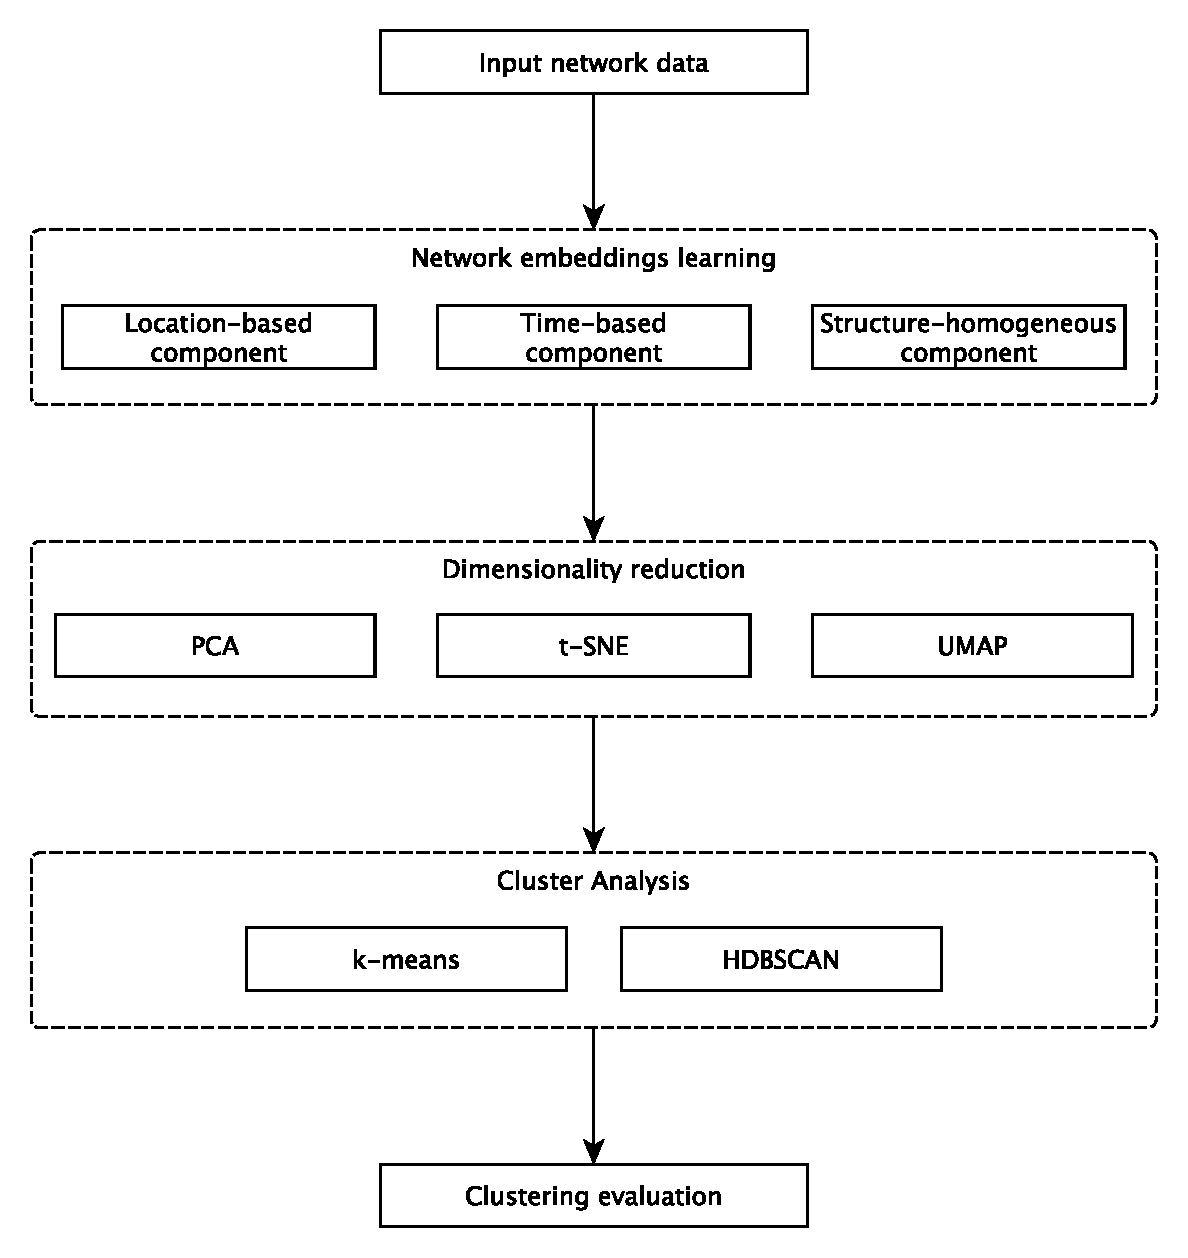
\includegraphics[width=0.7\textwidth]{images/Fig28.pdf}\\
	\caption{Concept of unsupervised data science pipeline for user segmentation in financial transaction networks.}
	\label{fig:Fig28}
\end{figure}

\section{Data preparation}
\label{Data Preparation}
Despite the input data structure is reasonably simple and requires the minimal feature set (sender, receiver, time), some pre-processing procedures have to be done as the input data preparation step for data analysis.

\subsection{Time classes}
The analysis involves time component. Transaction data sets usually contain timestamps for every transaction that are almost always unique with rare exceptions. As the goal is to place "time-similar" users closer together, i.e. the users acting at the same time period, it is reasonable to combine unique timestamps into periods. It allows to consider the users which act at the same time being more related to each other. To realize this strategy the entire time span has to be divided into consecutive time periods - time classes. Time classes have an equal length in time and do not overlap as~\autoref{fig:Fig29} shows. A particular time class can contain an arbitrary number of timestamps depending on the original data set and the time span split. The number of time classes is a user-defined parameter that can be tuned in the beginning. This pre-processing procedure results in every transaction belong to a particular class based on its timestamp.

\begin{figure}[!ht]
	\centering
	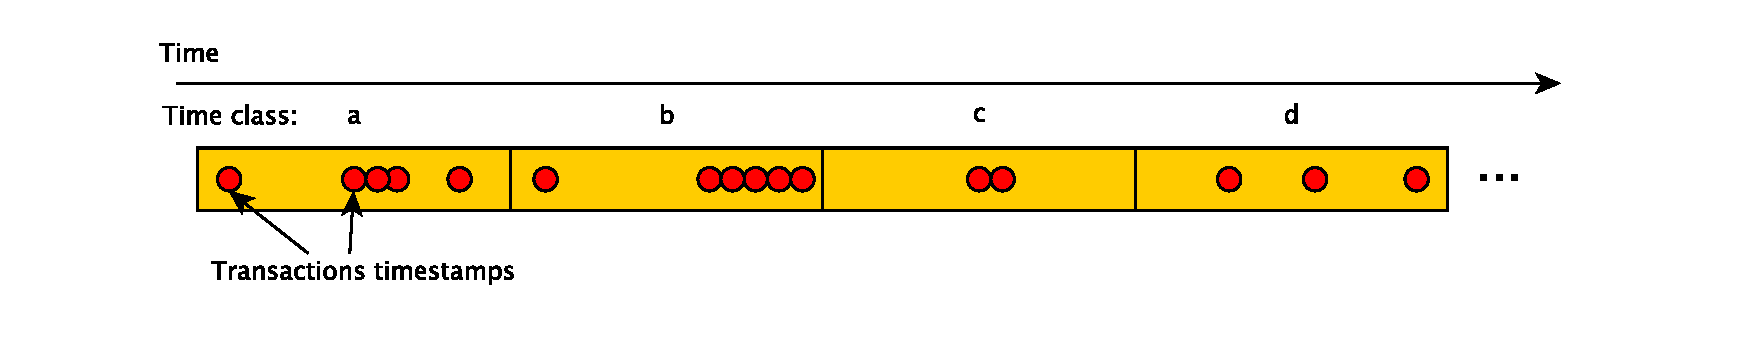
\includegraphics[width=0.95\textwidth]{images/Fig29.pdf}\\
	\caption{Transactions timestamps fall into the non-overlapping, equal-length time classes.}
	\label{fig:Fig29}
\end{figure}

\subsection{Degree classes}
Besides time, the analysis involves the degree of nodes in a network. 
It is easy and relatively fast to extract nodes' degree from a network of any size. Degree distribution of a real-world network commonly follows a Power law distribution. Thus, nodes with low degrees prevail over others. In contrast, a few nodes falling into the long tail of the distribution have high degrees and distributed sparsely. This fact suggests to group several high degrees to a degree class. A low degree can compose a degree class only by itself since a sufficient amount of nodes in a network have this degree. The number of nodes in the degree classes is determined based on considerations of the final clustering granularity. The more classes are allocated, the more clusters may be expected. 

Meaning of the global structural component is in distinguishing hubs of the highest degrees from end-points of degree one on a network's periphery. These two extrema lay on the opposite ends of the scale, while in-between there are two-degree nodes serving as bridges and other. This is another heuristic used for choosing degree classes. If there is a particular interest in participants with a certain number of established connections in a network, degree classes can be allocated in a way to capture them together. The number of degree classes is a user-defined parameter that can be tuned in the beginning. During this pre-processing procedure, every node is assigned to some degree class based on its degree.

\section{Automated feature learning framework}
\label{Automated Feature Learning Framework}
The previous section~\ref{Data Preparation} describes the data pre-processing procedures to comply with the input data format required by the automated feature learning framework. The network feature learning stage of the pipeline uses the Node2vec framework discussed in detail in the chapter~\ref{Node2vec}. The semi-random walk model of Node2vec generates ordered sequences of nodes' ids. However, unlike original Node2vec, the current framework modifies the sequences before submitting them as an input to a skip-gram model. Besides nodes' ids, the modified ordered sequences contain the time component represented by time classes of transactions and the global structural component defining the homogeneity of remote users over the network. The next two subsections will cover the imputations of time and degree to sequences of nodes' ids.

\subsection{Time component}
\label{Time component}
The Node2vec framework learns representations of network nodes in some feature space by sampling nodes' local neighbourhoods in the form of ordered sequences of nodes' ids. By nature, a time class in the prepared input data is defined for a transaction and not for a user represented by a network node. A transaction consists of two users: sender and receiver. To enable a skip-gram model to study a node representation from both its local neighbourhood and the time classes of transactions between nodes within this local neighbourhood, the ordered sequence should contain both nodes' ids and time classes.~\autoref{fig:Fig30} shows how an ordered sequence of nodes' ids alternated with time classes of intermediate transactions (bottom) can be obtained from a Node2vec semi-random walk sampled from a transaction graph (top).
\begin{figure}[!ht]
	\centering
	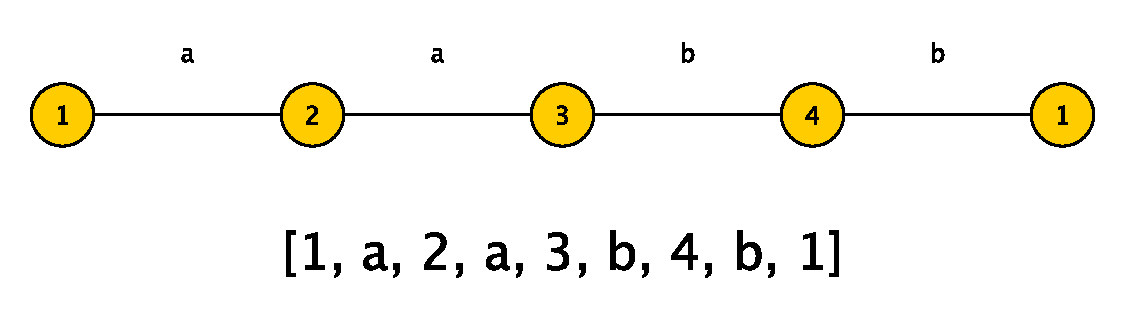
\includegraphics[width=0.5\textwidth]{images/Fig30.pdf}\\
	\caption{Top: Node2vec semi-random walk sampled from a transaction graph. Bottom: ordered sequence of nodes' ids and time classes of intermediate transactions.}
	\label{fig:Fig30}
\end{figure}

The ordered sequence on~\autoref{fig:Fig30} indicates that nodes 1, 2, 3, 4 are in the same neighbourhood, nodes 2 and 4 sent or received an asset at two different periods $a$ and $b$ respectively, nodes 1 and 3 were active both periods. 

However, real-world financial networks may contain transactions between the same sender and receiver which repeat after some time. Here the stochastic nature of the original Node2vec sampling facilitates the choice of the time class intervening between the same users. The framework stochastically generates many walks for a node's neighbourhood while the same nodes and edges may be traversed several times by different walks.~\autoref{fig:Fig31} shows this case along with the ordered sequence generated from a particular walk. The next walk may traverse nodes 2 and 3 by another edge and generate another time class between nodes 2 and 3 ([...2, a, 3,...]). This strategy reduces information loss and preserves time classes of all transactions between users.
\begin{figure}[!ht]
	\centering
	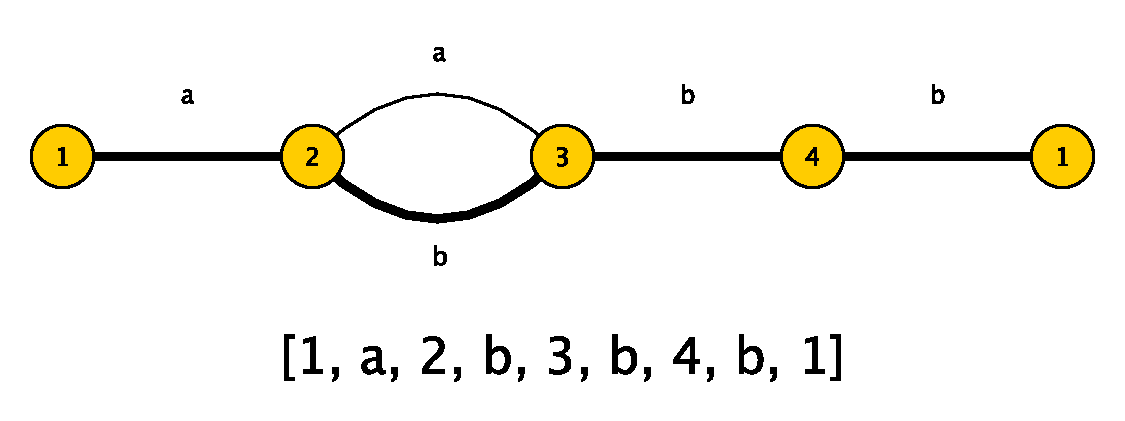
\includegraphics[width=0.5\textwidth]{images/Fig31.pdf}\\
	\caption{One of the possible way of traversing nodes for generating an ordered sequence of nodes' ids and time classes.}
	\label{fig:Fig31}
\end{figure}

\subsection{Global structural component}
\label{Global structural component}

The network embedding frameworks suffer from exploiting random or semi-random walk models as the main sampling strategy. Basically, it captures mostly proximity of nodes in a graph rather than the structural similarity of their neighbourhoods~\ref{Limitations of Node2vec}. Imputation of the global structural component is meant to overcome this shortcoming. It was inspired by the baseline idea of Role2vec framework~\cite{role2vec} which defines structural similarity by the node's membership to a certain structural class. Its authors Nesreen K. Ahmed et al. initially defined a set of structural classes and then assigned them to nodes based on their local structures regardless of their proximity in the graph. On the contrary, Node2vec structural similarity notion relies on the assumption that similar nodes are surrounded by similar context~\cite{role2vec}, means they have intersecting neighbourhoods.

The global node-based structural component can identify nodes playing similar structural roles (e.g. hub, bridge) in the different graph components and insert it to the ordered sequence of nodes' ids. ~\autoref{fig:Fig32} depicts a graph. Although red nodes belong to different components of the graph and are connected by the relatively long shortest path, they perform the same role of a local hub. Red nodes have relatively high degrees in the graph what makes them structurally similar to each other and different to other nodes in the graph.
\begin{figure}[!ht]
	\centering
	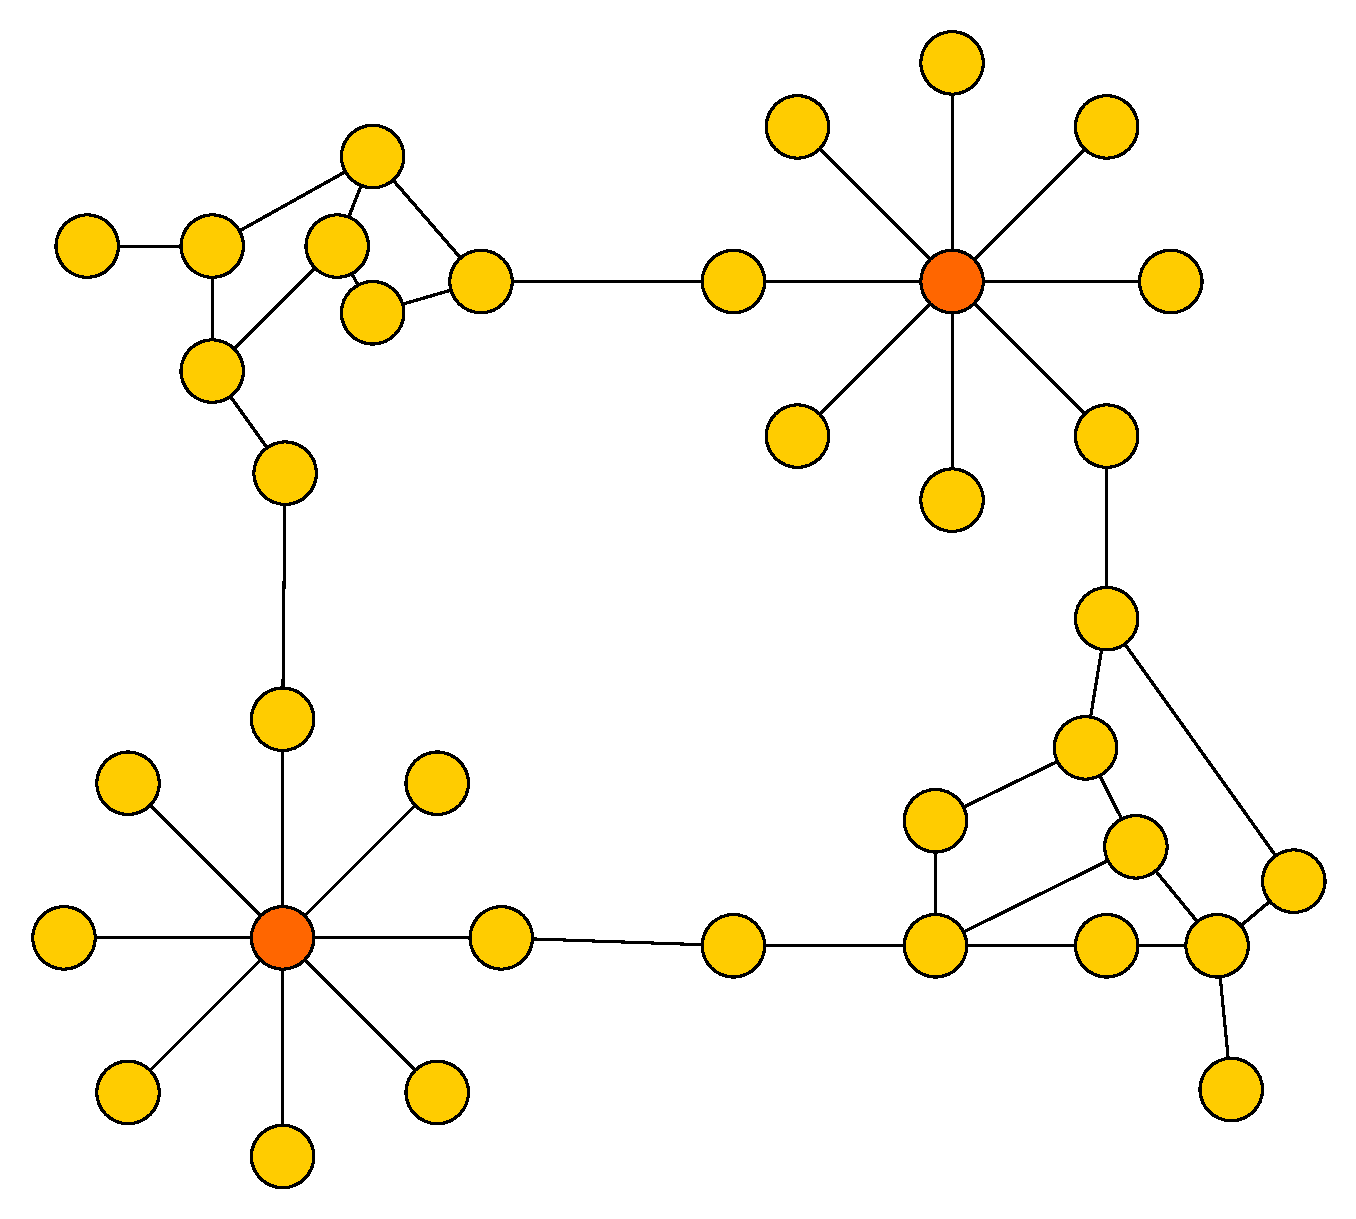
\includegraphics[width=0.3\textwidth]{images/Fig32.pdf}\\
	\caption{Red nodes belong to different components of the graph, whilst they are structurally similar and serve as local hubs.}
	\label{fig:Fig32}
\end{figure}

The imputation of the degree classes is similar to time classes imputation. The final sequences are the alternation of nodes' ids, acquired by the original Node2vec sampling and their degrees.

\section{Concept evaluation}
\label{Concept evaluation}
The overall concept is assessed by the goodness of the resulting clusters obtained from the final stage of the pipeline. Clustering results, in turn, are evaluated by a set of objective and quantitative measures. The majority of internal clustering evaluation measures are based on the intuition that clustering leads to the high similarity of the nodes within a cluster and low similarity between clusters. However, it is worth to mention that good scores on internal measures do not necessarily guarantee effective information retrieval from the original data.

~\autoref{tab:tab2} summarizes clustering evaluation indices used in the work. The list of metrics was inspired by~\cite{liu2010understanding} and~\cite{kovacs2005cluster}, their meanings along with calculation methods were explained in~\ref{Cluster evaluation strategies}.

\begin{table}[H]
\begin{center}
\begin{tabular}{ | m{0.7em} | m{8cm}| m{1.5cm} | m{2.6cm} |} 
\hline
\textbf{\#} & \textbf{validity measure} & \textbf{notation} & \textbf{optimal value} \\ 
\hline
1 & Root-mean-square standard deviation index & \textit{RMSSTD} & min \\ 
\hline
2 & R-square index & \textit{RS} & max \\ 
\hline
3 & SD Validity index  & \textit{SD} & min \\ 
\hline
4 & S\_Dbw Validity index   & \textit{S\_Dbw} & min \\ 
\hline
5 & Silhouette coefficient & \textit{SC} & max \\ 
\hline
6 & Davies–Bouldin index & \textit{DB} & min \\
\hline
7 & Dunn index & \textit{D} &  max \\
\hline
8 & Calinski-Harabasz index & \textit{CH} &  max \\
\hline
\end{tabular}
\caption {Internal clustering validation measures}
\label{tab:tab2}
\end{center}
\end {table}

These particular clustering evaluation measures are used for two main purposes.
\begin{enumerate}
  \item Although clustering results are affected to a large extent by user-defined input hyperparameters, there is no conventional way of choosing such hyperparameters. The above evaluation measures facilitate the tuning of clustering hyperparameters. Cluster analysis runs several times for each value of slightly changing hyperparameter or combination of hyperparameters. Each run generates a set of evaluation measures values. A clustering and its hyperparameter with the best measures' values are considered as the best set of clusters and the optimal hyperparameter.
  \item The pipeline is constructed as a branching tree. At the last stage, it outputs several clustering results from different branches which contain different cluster analysis techniques. It is crucial to have a unified scale for comparison of such results. The internal clustering evaluation measures in~\autoref{tab:tab2} are used to compare results from the different pipeline's branches and to find the best cluster set.
\end{enumerate}

\section{Summary}
This chapter covered the aim of the concept and its form - data science pipeline. Additionally, to three stages of the pipeline, it provided insights into data preparation and evaluation procedures. The main part of the chapter was devoted to the unique way of sampling from networks in the automated feature learning process. The proposed strategy in~\ref{Automated Feature Learning Framework} benefits from nodes' local neighbourhoods, time, and global structural components all in one. It is meant to enrich the learning capabilities of the framework, which will reveal in cluster analysis at the final stage.

The upcoming chapter leads through implementation details and introduces some third-party frameworks exploited at different stages of the developed pipeline.


